% DPF 09 talk on strangeness in nucleon

\documentclass[10pt]{beamer}
\usefonttheme{professionalfonts} % using non standard fonts for beamer
\usefonttheme{serif} % default family is serif
\usepackage{amsmath}
\usepackage{array}
\usepackage{mathtools}
%\documentclass[12pt]{beamerthemeSam.sty}
\usepackage{epsf}
%\usepackage{pstricks}
%\usepackage[orientation=portrait,size=A4]{beamerposter}
\geometry{paperwidth=160mm,paperheight=120mm}
%DT favorite definitions
\def\LL{\left\langle}	% left angle bracket
\def\RR{\right\rangle}	% right angle bracket
\def\LP{\left(}		% left parenthesis
\def\RP{\right)}	% right parenthesis
\def\LB{\left\{}	% left curly bracket
\def\RB{\right\}}	% right curly bracket
\def\PAR#1#2{ {{\partial #1}\over{\partial #2}} }
\def\PARTWO#1#2{ {{\partial^2 #1}\over{\partial #2}^2} }
\def\PARTWOMIX#1#2#3{ {{\partial^2 #1}\over{\partial #2 \partial #3}} }

\def\rightpartial{{\overrightarrow\partial}}
\def\leftpartial{{\overleftarrow\partial}}
\def\diffpartial{\buildrel\leftrightarrow\over\partial}

\def\BI{\begin{itemize}}
\def\EI{\end{itemize}}
\def\BE{\begin{displaymath}}
\def\EE{\end{displaymath}}
\def\BEA{\begin{eqnarray*}}
\def\EEA{\end{eqnarray*}}
\def\BNEA{\begin{eqnarray}}
\def\ENEA{\end{eqnarray}}
\def\EL{\nonumber\\}



\newcommand{\etal}{{\it et al.}}
\newcommand{\gbeta}{6/g^2}
\newcommand{\la}[1]{\label{#1}}
\newcommand{\ie}{{\em i.e.\ }}
\newcommand{\eg}{{\em e.\,g.\ }}
\newcommand{\cf}{cf.\ }
\newcommand{\etc}{etc.\ }
\newcommand{\atantwo}{{\rm atan2}}
\newcommand{\Tr}{{\rm Tr}}
\newcommand{\dt}{\Delta t}
\newcommand{\op}{{\cal O}}
\newcommand{\msbar}{{\overline{\rm MS}}}
\def\chpt{\raise0.4ex\hbox{$\chi$}PT}
\def\schpt{S\raise0.4ex\hbox{$\chi$}PT}
\def\MeV{{\rm Me\!V}}
\def\GeV{{\rm Ge\!V}}

%AB: my color definitions
%\definecolor{mygarnet}{rgb}{0.445,0.184,0.215}
%\definecolor{mygold}{rgb}{0.848,0.848,0.098}
%\definecolor{myg2g}{rgb}{0.647,0.316,0.157}
\definecolor{abtitlecolor}{rgb}{0.0,0.255,0.494}
\definecolor{absecondarycolor}{rgb}{0.0,0.416,0.804}
\definecolor{abprimarycolor}{rgb}{1.0,0.686,0.0}
\definecolor{Red}           {cmyk}{0,1,1,0}
\definecolor{Grey}           {cmyk}{.7,.7,.7,0}
\definecolor{Lg}           {cmyk}{.4,.4,.4,0}
\definecolor{Blue}          {cmyk}{1,1,0,0}
\definecolor{Green}         {cmyk}{1,0,1,0}
\definecolor{Brown}         {cmyk}{0,0.81,1,0.60}
\definecolor{Black}         {cmyk}{0,0,0,1}

\usetheme{Madrid}


%AB: redefinition of beamer colors
%\setbeamercolor{palette tertiary}{fg=white,bg=mygarnet}
%\setbeamercolor{palette secondary}{fg=white,bg=myg2g}
%\setbeamercolor{palette primary}{fg=black,bg=mygold}
\setbeamercolor{title}{fg=abtitlecolor}
\setbeamercolor{frametitle}{fg=abtitlecolor}
\setbeamercolor{palette tertiary}{fg=white,bg=abtitlecolor}
\setbeamercolor{palette secondary}{fg=white,bg=absecondarycolor}
\setbeamercolor{palette primary}{fg=black,bg=abprimarycolor}
\setbeamercolor{structure}{fg=abtitlecolor}

\setbeamerfont{section in toc}{series=\bfseries}

%AB: remove navigation icons
\beamertemplatenavigationsymbolsempty
\title{
  \textbf {Introduction}\\
%\centerline{}
%\centering
%\vspace{-0.0in}
%\includegraphics[width=0.3\textwidth]{propvalues_0093.pdf}
%\vspace{-0.3in}\\
%\label{intrograph}
}

\author[W. Freeman] {Physics 211\\Syracuse University, Physics 211 Spring 2016\\Walter Freeman}

\date{\today}

\begin{document}

\frame{\titlepage}

\frame{\frametitle{\textbf{Welcome!}}

\Huge
\begin{center}
Physics 211 \\
Forces and Motion\\

\bigskip

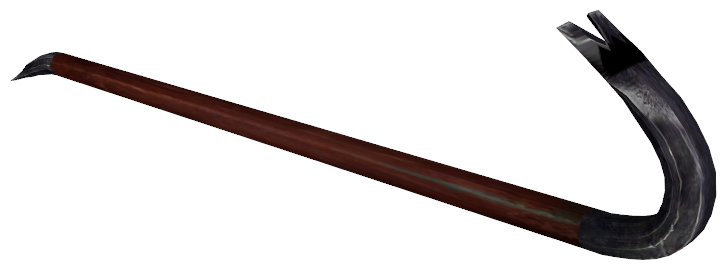
\includegraphics[width=0.3\textwidth]{crowbar.jpg}\\
\Large

\bigskip

Dr. Walter Freeman (suphysics211@gmail.com), professor\\
Francesco Serafin (fserafin@syr.edu), lead TA\\


\bigskip

Course webpage:

\Huge
http://suphysics211.wikispaces.com
\end{center}
}

\frame{\frametitle{\textbf{Overview of today}}

\Large

\begin{itemize}
\item{Introduction to physics and mechanics}
\item{Course organization / syllabus}
\item{How to succeed in this course}
\item{{\color{Green}} Describing motion: position and velocity}
\end{itemize}
}

\frame{\frametitle{\textbf{So what is this class?}}

\Large
\begin{center}
Physics: what are the fundamental laws of nature?

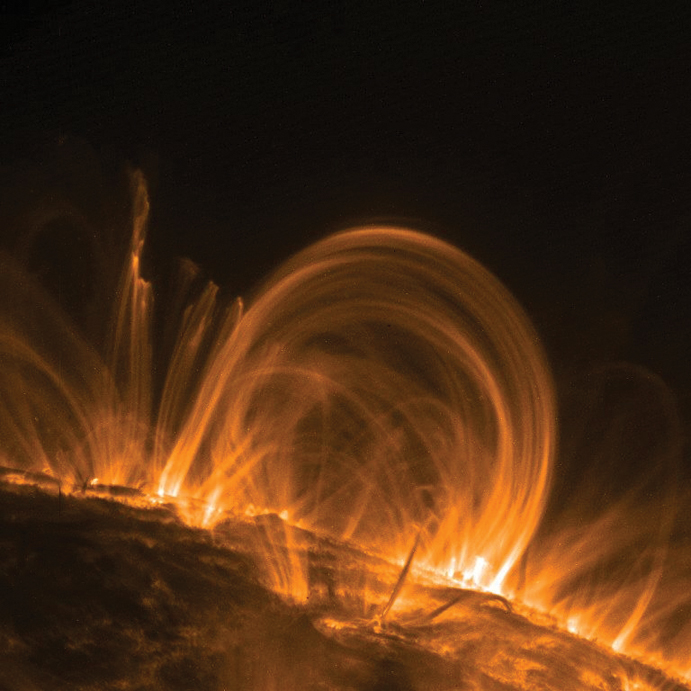
\includegraphics[width=0.27\textwidth]{sun.jpg}
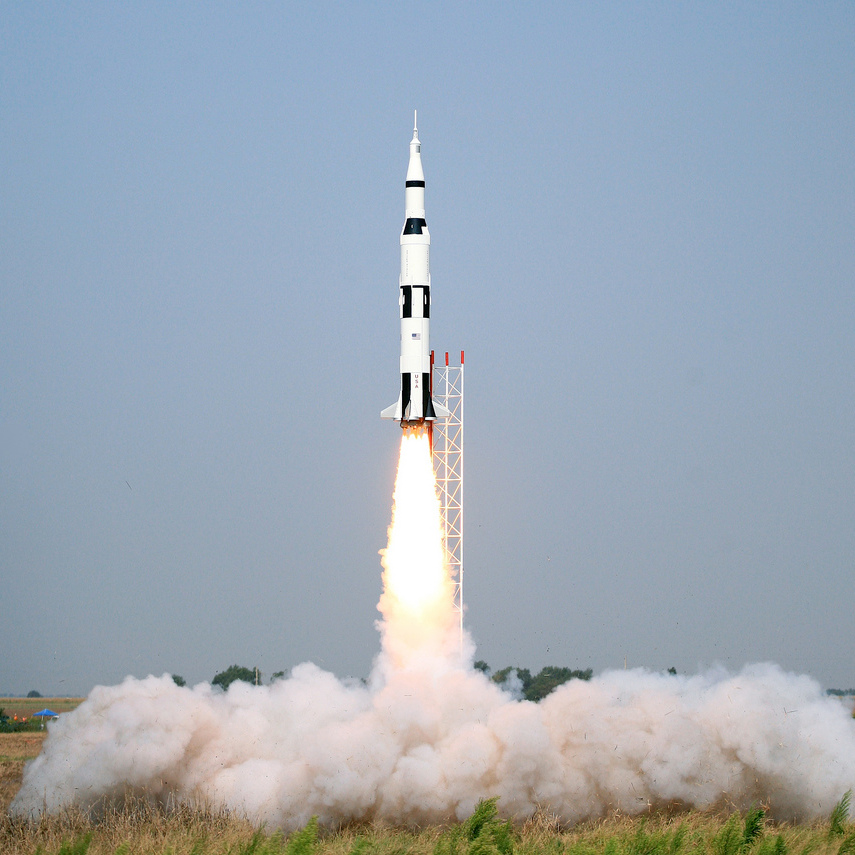
\includegraphics[width=0.27\textwidth]{rocket.jpg}
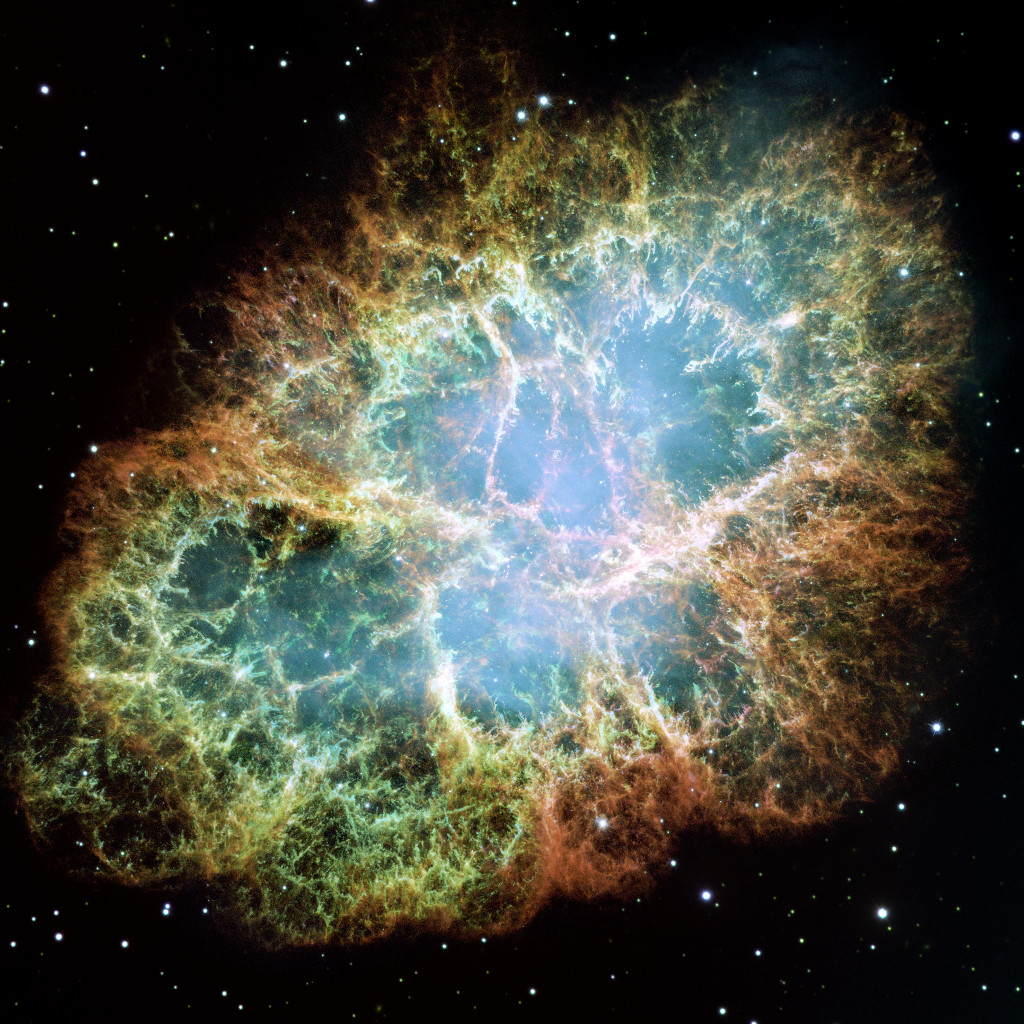
\includegraphics[width=0.27\textwidth]{crab-nebula.jpg}\\
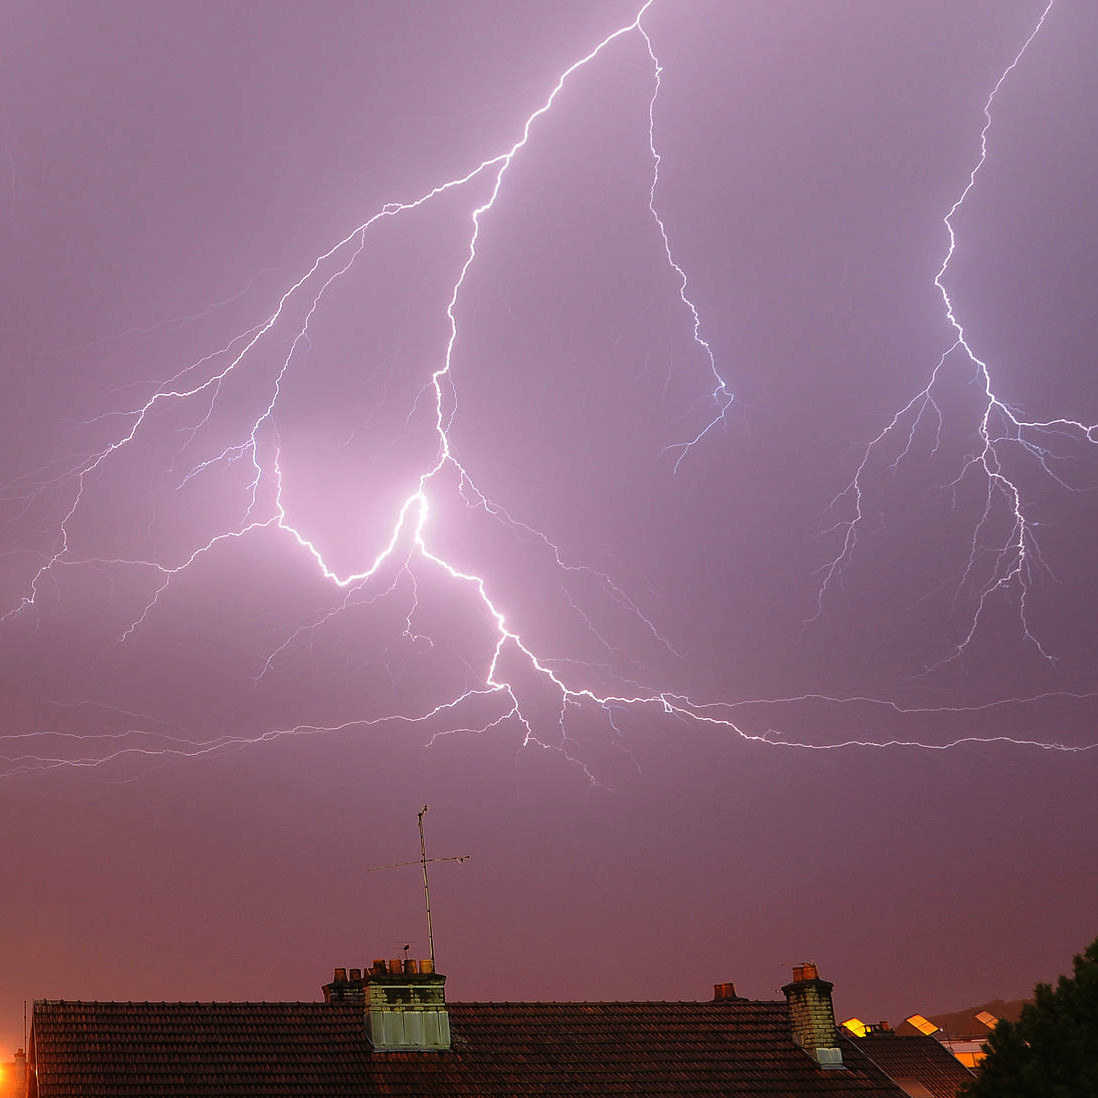
\includegraphics[width=0.27\textwidth]{lightning.jpg}
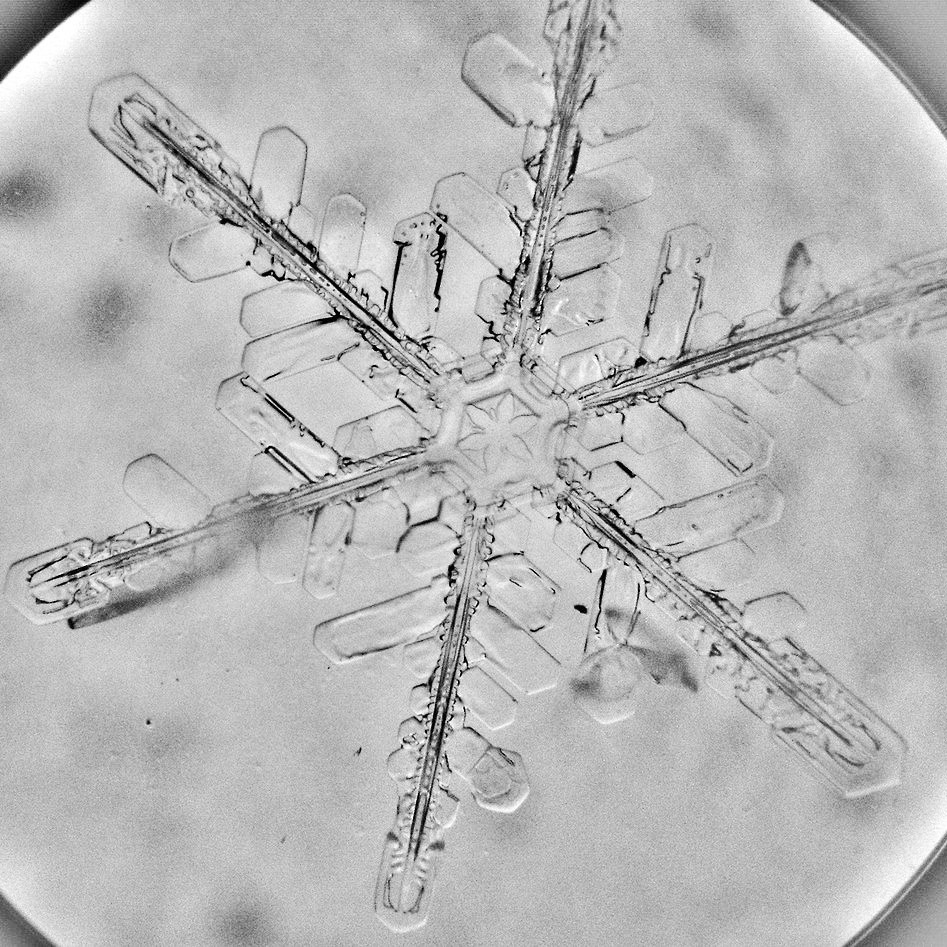
\includegraphics[width=0.27\textwidth]{snowflake.jpg}
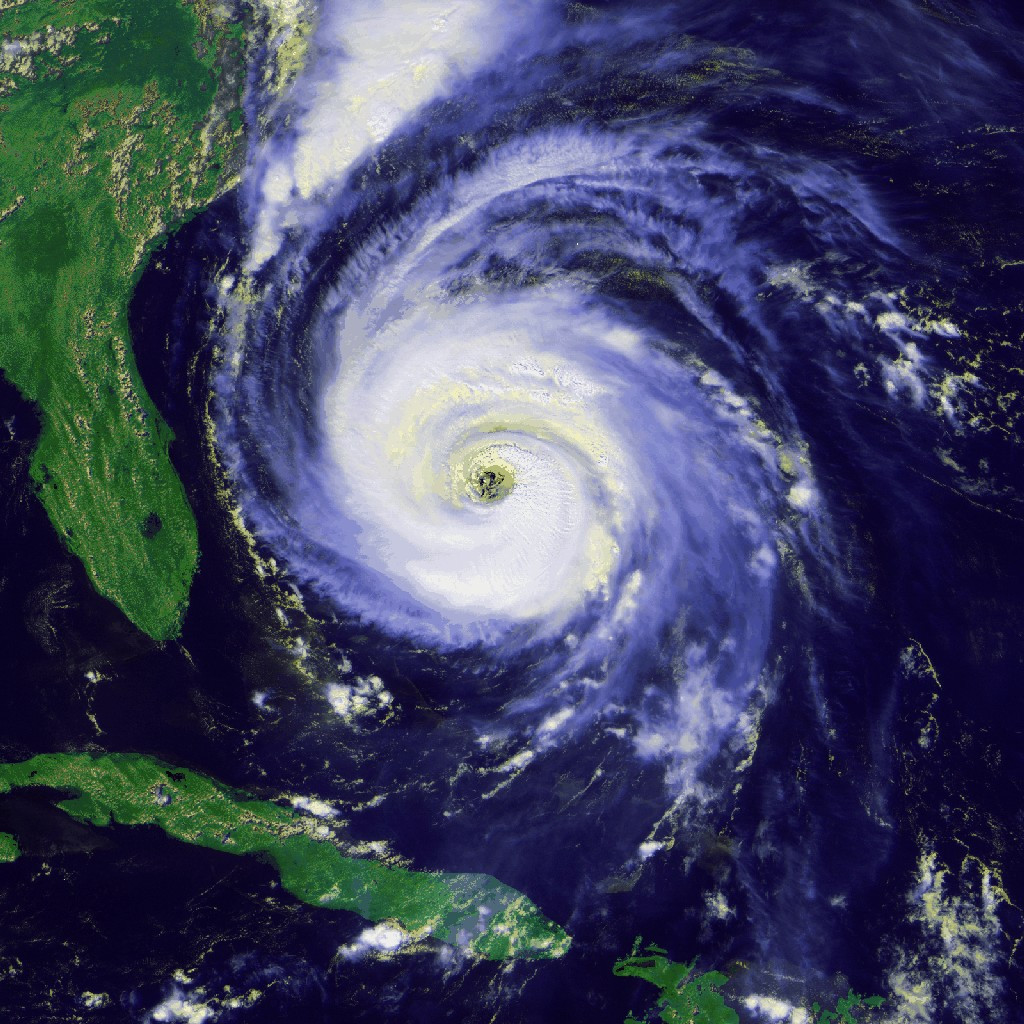
\includegraphics[width=0.27\textwidth]{hurricane.jpg}\\
These phenomena are all governed by the {\it same few principles}.
\end{center}
}

\frame{\frametitle{\textbf{Mechanics}}

The most fundamental question physics asks:

\bigskip

\Large \centerline{\color{Red}``Why do things move in the ways that they do?''}


\bigskip

\normalsize

The answer is given by Isaac Newton's second law of motion:


\bigskip

\begin{center}
\Large {\color{Blue} ``Objects accelerate when pushed by forces; they accelerate in the direction of the force, proportional to the size of the force divided by their mass.''}
\end{center}
\normalsize


\bigskip

That's it. We will spend much of our class talking about the meaning and consequences of this one statement.

}

\frame{\frametitle{\textbf{The physicist's eye}}

\large

Physics is about {\color{Blue} understanding complicated things in terms of simple pieces}, like Newton's law.

\pause
\bigskip

The perspective of physics is one that looks at a situation and asks:

\begin{itemize}
\item{``What phenomena are involved in this thing?''}
\item{``How do they interact to determine its behavior?''}
\end{itemize}
\pause
\bigskip

In this class, you'll learn about some of those simple pieces, but that's not the important thing.

\bigskip

You'll also learn the skill of asking those two questions, and develop {\color{Blue}a physicist's perspective for solving problems}.

\bigskip

This will serve you well in whatever field you pursue, since the ability to quickly look at a problem and understand the crucial 
elements is universally helpful.

%\begin{center}
%\begin{tabular}{|p{3cm}|p{3cm}|}
%\hline
%Things known & Things needed \\ 
%\hline
%Assumptions & Representations \\
%\hline
%\end{tabular}
%\end{center}

}

\frame{\frametitle{\textbf{What is this (and how does it work)?}}
\centerline{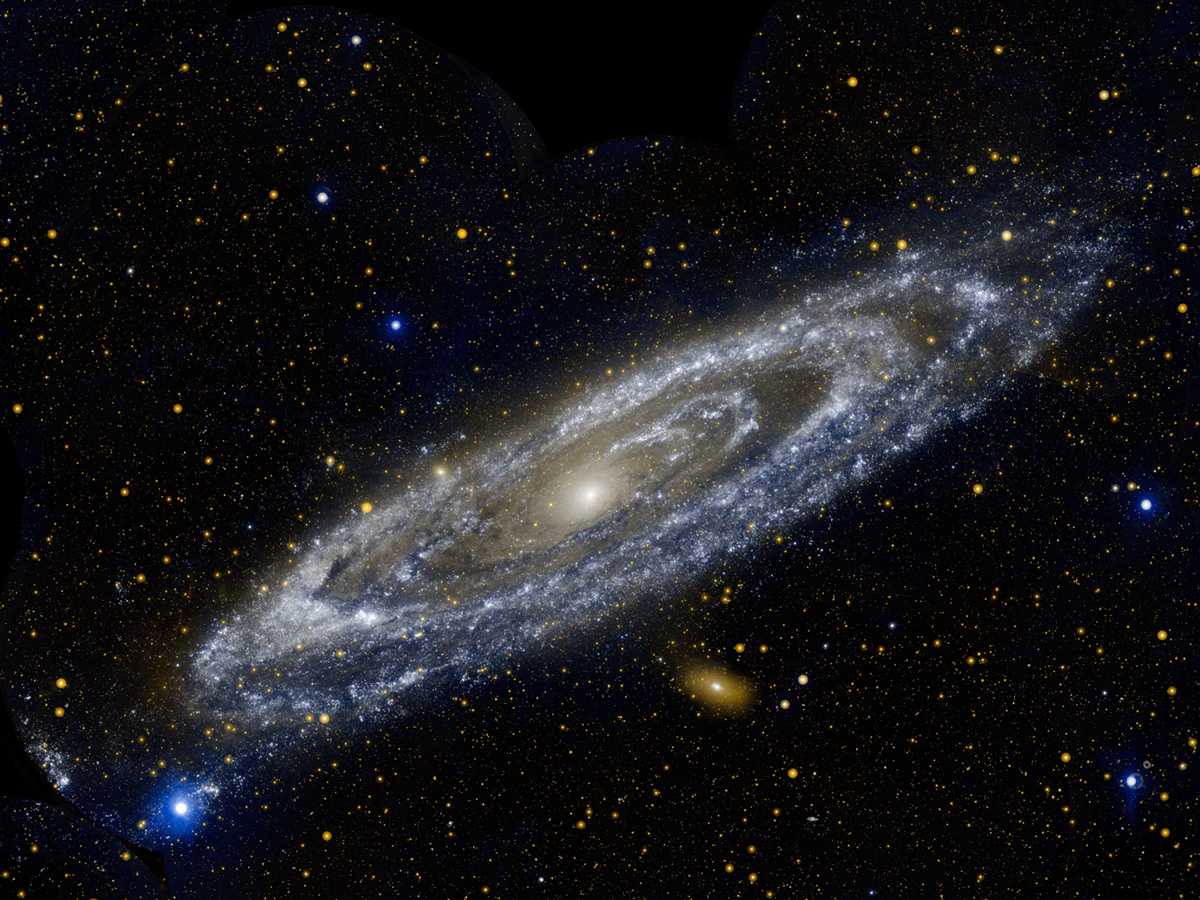
\includegraphics[width=0.8\textwidth]{andromeda.jpg}}
}

\frame{\frametitle{\textbf{How it works: the physicist's perspective}}
\pause

\begin{itemize}
\item{Lots and lots of stars...}
\item{They exert forces on each other through gravity}
\pause
\item{Those forces cause accelerations: $\vec F = m \vec a$ (don't worry, you'll learn about the arrows)}
\item{Those accelerations then affect the stars' motion}
\pause
\begin{itemize}
\item{The accelerations change the stars' speed and direction of travel}
\end{itemize}
\item{Too many stars to do with pen and paper...}
\pause
\item{\href{https://youtu.be/PrIk6dKcdoU}{... but a computer can do it!} (youtube link)}
\end{itemize}
}

\frame{\frametitle{\textbf{Course structure and syllabus review}}
\centerline{\Large{Three broad sections:}}
\bigskip
\Large
\begin{enumerate}
\item{Kinematics (understanding the right hand side of $\vec F=m \vec a$)}
\begin{itemize}
\item{How do we describe motion?}
\item{How do an object's position, velocity, and acceleration relate?}
\item{{\color{Red}What about rotational motion?}}
\item{How do we deal with things in two or three dimensions?}
\end{itemize}
\pause
\item{Forces and motion (both sides of $\vec F=m \vec a$)}
\begin{itemize}
\item{What kinds of forces are there?}
\item{{\color{Red}Torque: a rotational counterpart to force, with an equivalent to $\vec F = m \vec a$}}
\item{Understanding different physical situations using $\vec F = m \vec a$}
\item{Collisions and momentum: taking the integral of $\vec F = m \vec a$}
\end{itemize}
\pause
\item{Two more topics}
\begin{itemize}
\item{Energy: a way to simplify solving $\vec F = m \vec a$ when you don't care about time}
\item{{\color{Red}How do forces cause torques?}}
\end{itemize}
\end{enumerate}
}

\frame{\frametitle{\textbf{Clickers}}
Starting next week, we'll start using clickers in class, and the week after that,
your participation in clicker questions wil be graded.

\begin{itemize}
\item{Clickers are little radio devices you can use to answer questions in class}
\item{You can also use a smartphone or tablet}
\end{itemize}

\bigskip

You will need to either:
\begin{itemize}
\item{Buy a Turning Technologies clicker from the bookstore or elsewhere, or}
\item{... download the ResponseWare app on your smartphone, then set up an account and buy a license
for \$20 (cheaper than a clicker)}
\end{itemize}
}

\frame{\frametitle{\textbf{Mastering Physics}}
\large
Mastering Physics is an online homework system. Due to negative feedback from students I
don't require it, but it is still for sale in the bookstore; you do not need to buy it.}

\frame{\frametitle{\textbf{Grading}}
\begin{itemize}
\item{Homework: 30\% (submitted to your recitation TA)}
\item{Exams: 50\%}
\begin{itemize}
\item{Each of the three sections has an exam}
\item{{\color{Red}Every exam has a makeup given two weeks later}}
\item{{\color{Green}You can take both and keep the higher grade}}
\end{itemize}
\item{Class participation (clicker questions): 5\%}
\item{Computational projects (mostly done in recitation): 10\%}
\item{Recitation attendance: 5\%}
\item{Up to 2\% extra credit for participation in course Facebook group}
\item{Up to 2\% extra credit for exceptional participation in recitations, etc.}
\EI

\bigskip
\bigskip
\bigskip

The makeup for the third exam will be given during the final exam period. {\it There is no separate final.}

}

\frame{\frametitle{\textbf{Recitations}}
\BI
\large
\item{Discussion sections led by your TA}
\item{Homework is submitted and returned in recitation}
\item{{\bf Crucial} for your success in this class}
\BI
\large
\item{Ask general questions to your TA and your peers}
\item{Work on homework questions in groups}
\item{Work on recitation worksheets/questions, or problems from the workbook}
\item{{\color{Blue} Work on computational assignments (introduced next week)}}
\EI
\item{Physics is not about how much you know -- it's about {\bf what you can do}}
\item{This class isn't about amassing facts; it's about solving problems}
\item{This requires practice, and the recitations (and the homework) are where you get it}
\item{The TA's this year are a fantastic bunch; make use of them!}
\EI
}

\frame{\frametitle{\textbf{The course webpage and Facebook page}}
\large
\BI
\item{All notes, etc., will be posted on http://suphysics211.wikispaces.com (not Blackboard)}
\item{I will also post course announcements there}
\item{The syllabus is posted there}
\item{... so is some information on how to succeed in this class; you should read it!}
\EI
\bigskip
\bigskip
\BI
\item{There is also a course Facebook page at https://www.facebook.com/groups/1553254954993837/}
\item{... or search ``Syracuse University Physics 211, Spring 2016''}
\item{Joining the group doesn't mean anyone else can see your private posts etc.}
\item{This is a great place to ask questions, get advice, and collaborate with your classmates}
\item{Up to 2\% extra credit for those who help their peers}
\EI
}

\frame{\frametitle{\textbf{How to do well in this class (important!)}}
\Large
\centerline{This class isn't about learning facts or memorizing equations!}
\pause
\bigskip
\large
In this class, I hope you will:
\BI
\item{... learn to look at moving things around you in a new, rigorous way}
\pause
\item{... learn to solve problems by taking them apart, understanding the parts, and putting them back together again}
\pause
\item{... learn to translate between and combine verbal, visual, and mathematical descriptions of things, while still being precise}
\pause
\EI

\centerline{These things are skills, and they all require practice}
\centerline{... but they also require you to ask questions and ask for guidance!}
}

\frame{\frametitle{\textbf{How to do well in this class: ask for guidance!}}
\Large
\begin{center}
Some students might come to class, write down everything,
go home and review, and then spend hours alone working on the homework...
\end{center}
\pause

\bigskip

\centerline{... but this is not the best way to learn skills! Instead, I hope you will:}
\medskip

\large
\BI
\item{Interrupt me in class and ask questions}
\item{Ask me questions by email to {\bf suphysics211@gmail.com}}
\BI
\normalsize
\item{I am often by a computer and you will often get a quick reply}
\item{You can take cellphone pictures of work and email them to me, too}
\EI
\item{Ask questions on the Facebook group}
\item{Come work with me and with your peers in my office hours}
\item{Do your homework in the Physics Clinic when you can}
\EI
}

\frame{\frametitle{\textbf{Metaphors: sports and music}}
\large

Learning physics is like learning to play a musical instrument.

\bigskip

The hard part isn't learning the notes -- it's being able to play them, and tell a story with them.

\bigskip

How does studying the piano work?

\begin{itemize}
\item{Your teacher shows you a few techniques, and gives you a piece to learn to play}
\item{You take it home, practice it, and get stuck on difficult parts}
\item{You ask your teacher for advice; she guides you}
\item{You practice some more}
\item{You repeat the previous steps until you've mastered the technique and the music}
\end{itemize}

\bigskip

Learning a sport works the same way.

\bigskip

Physics is like this. We don't expect you to master everything immediately; physics takes practice, and it's
okay to get stuck and ask questions. In fact, it's what I expect!
}

\frame{\frametitle{\textbf{The Physics Clinic}}
\large
The Clinic is in room 112; it's a large room with tables, boards, and (usually) a graduate teaching 
assistant.

\bigskip

You can go there whenever the building is open to work in groups on your homework, and
ask each other and the GTA for help.


\bigskip

I also hold my office hours there.

\bigskip

This is an excellent resource for you to use; why do your homework alone when you can work
with your peers and instructors?
}

\frame{\frametitle{\textbf{Office hours}}
\Large
In the Physics Clinic:
\BI
\item{Mondays: 10-12 AM}
\item{Tuesdays: 4-6 PM}
\item{Thursdays: 1:30-3:30 PM}
\item{Fridays: 2:00-4:00 PM}
\EI

or by appointment.  
\bigskip
\bigskip

Outside these times you might find me in the Clinic or in my office in room 215.
}

\frame{\frametitle{\textbf{The beginning: describing motion (1-D)}}
\large
Recall that at first, we are only concerned with describing motion.

\bigskip

\BI
\large
\item{Most fundamental question: ``where is the object I'm talking about?''}
\item{Quantify position using a ``number line'' marked in meters:}
\BI
\normalsize
\item{Choose one position to be the origin (``zero'') -- anywhere will do}
\item{Choose one direction to be positive}
\item{Measure everything relative to that}
\item{Can measure in any convenient units: centimeters, meters, kilometers...}
\EI

\bigskip

\item{You're used to this already, perhaps:}
\BI
\normalsize
\item{Mile markers on highways}
\item{Yard lines in American football}
\EI
\EI
}

\frame{\frametitle{\textbf{Equations of motion}}
\large
Complete description of motion: ``Where is my object at each point in time?''

\bigskip

This corresponds to a mathematical function. Two ways to represent these. Suppose I drop
a ball off a building, putting the origin at the ground and calling ``up'' the positive direction:

\bigskip
\bigskip

\begin{columns}
\column{0.5\textwidth}
\centerline {\color{Red}\Large Graphical representation}
\column{0.5\textwidth}
\centerline{\color{Blue} \Large Algebraic representation}
\end{columns}

\bigskip

\begin{columns}
\column{0.5\textwidth}

\centerline{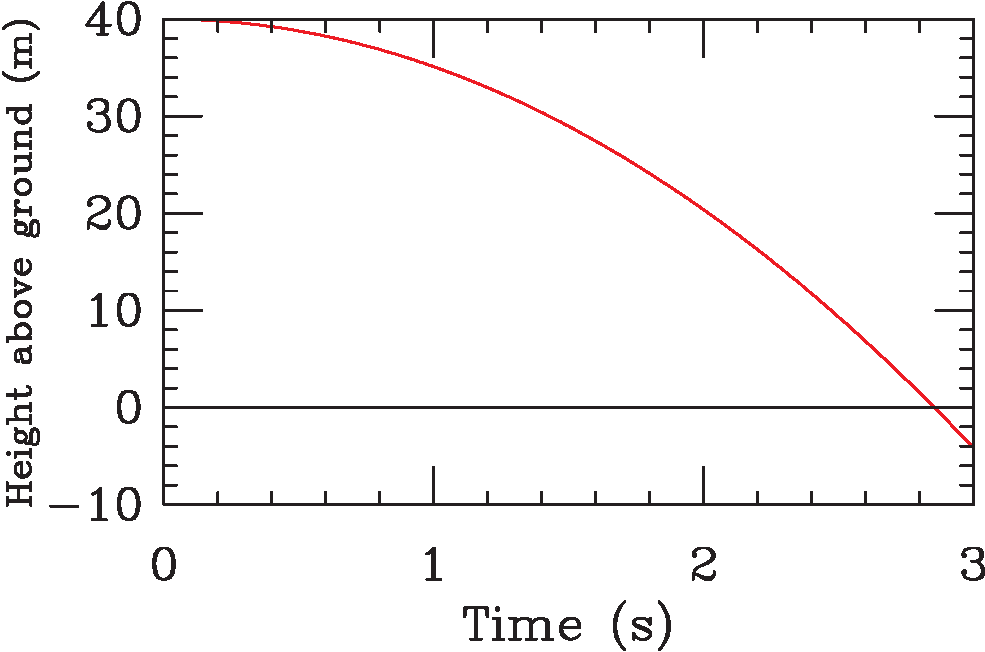
\includegraphics[width=0.7\textwidth]{falling-crop.pdf}}

\column{0.5\textwidth}
\color{Blue}
$$y(t) = (40 \,{\mathrm m}) - C t^2$$ \\
(C is some number; we'll learn what it is Thursday)

\end{columns}

\bigskip

\centerline{Both let us answer questions like ``When does the object hit the ground?''}

\bigskip

\begin{columns}
\column{0.5\textwidth}
\centerline {\color{Red}\large $\rightarrow$ ... the curve's x-intercept}
\column{0.5\textwidth}
\centerline{\color{Blue} \large $\rightarrow$ ... when $y(t)=0$}
\end{columns}

}

\frame{\frametitle{\textbf{Velocity: how fast position changes}}
\large
The slope of the position vs. time curve has a special significance. Here's one with a constant slope:

\medskip

\centerline{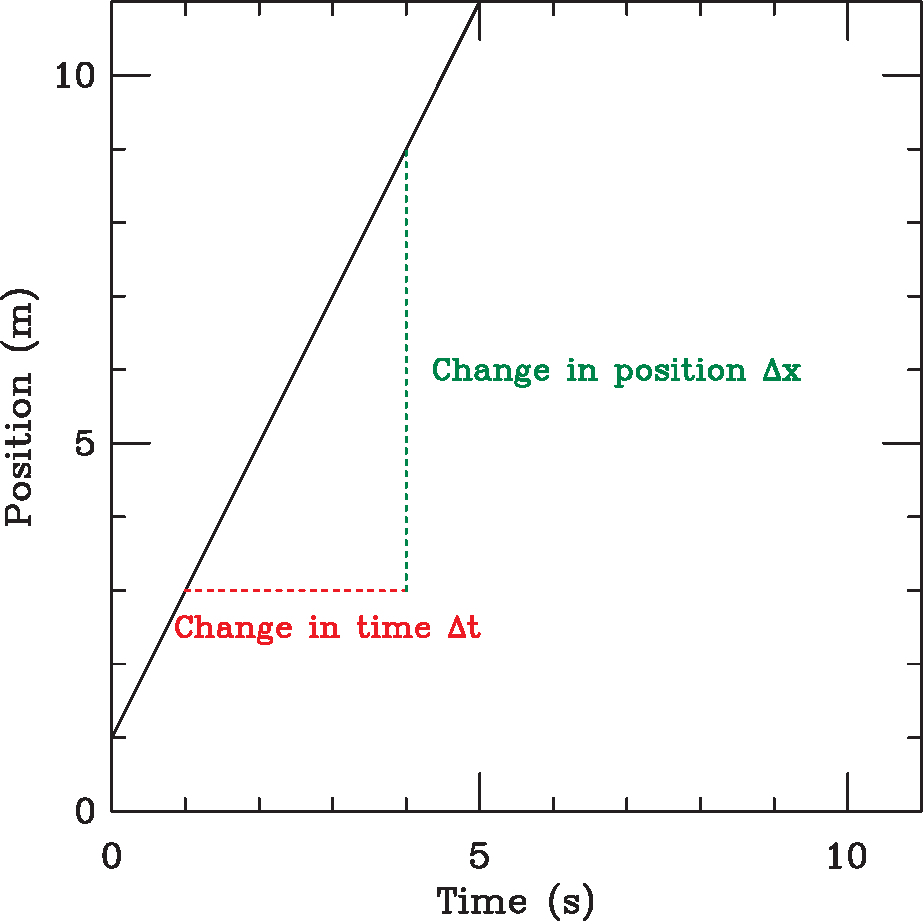
\includegraphics[width=0.4\textwidth]{constant-v-crop.pdf}}

\bigskip

\pause

Slope is $\frac{{\rm rise}}{{\rm run}}$ = $\frac{\Delta x}{\Delta t}$ = $\frac{2\,\rm m}{1 \, \rm s}$ = 2 meters per second (positive;
it could well be negative!)

\bigskip \pause

{\color{Red} $\rightarrow$ The slope here -- change in position over change in time -- is the {\bf velocity}!} Note that it can be
positive or negative, depending on which way the object moves.

}


\frame{\frametitle{\textbf{Constant-velocity motion: connecting graphs to algebra}}
\large
If an object moves with constant velocity, its position vs. time graph is a line:

\medskip

\centerline{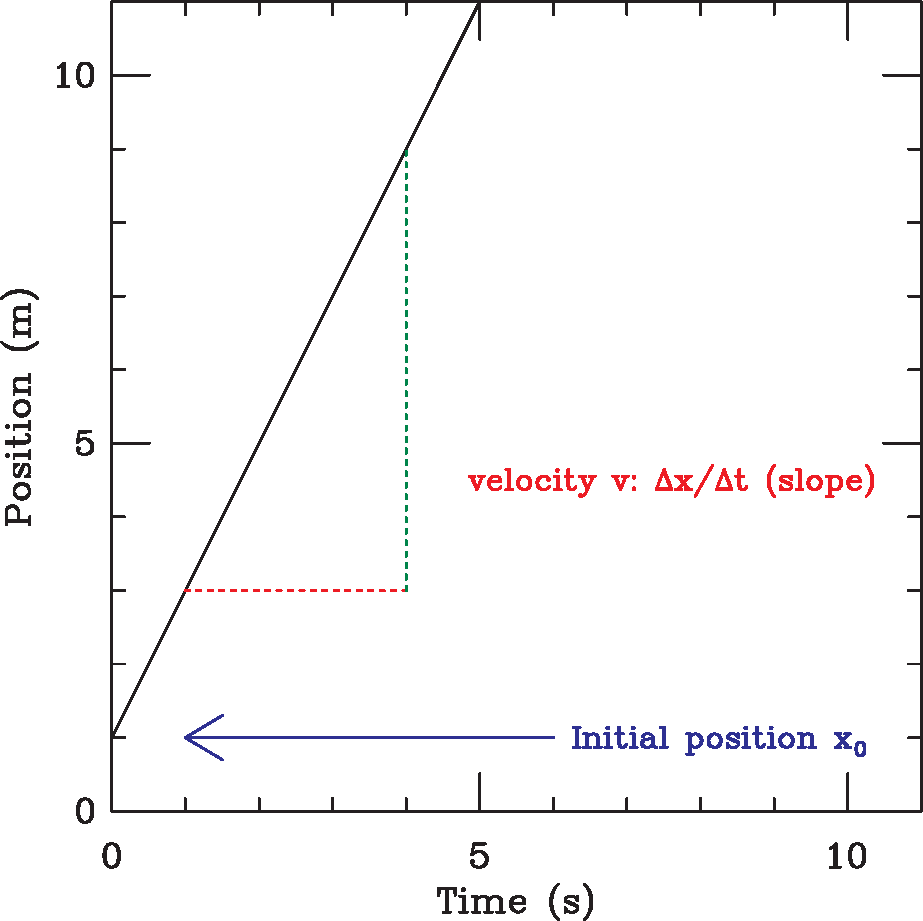
\includegraphics[width=0.4\textwidth]{constant-v-2-crop.pdf}}

We know the equation of a straight line is is $x = mt + b$ (using $t$ and $x$ as our axes).

\BI
\item{$m$ is the slope, which we identified as the velocity}
\item{$b$ is the vertical intercept, which we recognize as the value of $x$ when $t=0$}
\EI

We can thus change the variable names to be more descriptive:

\bigskip

\centerline{\Large{{\color{Red} $x(t) = vt + x_0$} (constant-velocity motion)}}

}

\frame{\frametitle{\textbf{Going from ``equations of motion'' to answers}}

\large

{\color{Red}$x(t) = vt + x_0$} is called an {\it equation of motion}; in this case, it is valid for constant-velocity motion.

\medskip

It gives you the same information as a position vs. time graph, but in algebraic form.

\bigskip
\bigskip

\normalsize

To solve real problems, we need to be able to translate physical questions into algebraic statements:
\bigskip
\bigskip

\BI
\item{``If a car starts at milepost 30 and drives at 50 mph, where is it an hour later?''}
\pause
\BI
\item{Using $x(t) = x_0 + vt$, with $x_0=30\, {\rm mi}$ and $v = 50 \frac{\rm mi}{\rm hr}$, calculate $x$ at $t=1\, {\rm hr}$}
\EI
\pause
\item{``When does a falling object hit the ground?''}
\pause
\BI
\item{If the ground is at $y=0$, then we ask: ``What is the value of $t$ when $y=0$?''}
\EI
\pause
\item{``When do two moving objects meet?''} 
\pause
\BI
\item{Write down $x_1(t)$ and $x_2(t)$, then ask ``At what time does $x_1 = x_2$?''}
\EI
\EI
}

\frame{\frametitle{\textbf{A rough problem-solving guide for constant-velocity motion}}

\large

A general framework for solving constant-velocity problems algebraically:

\begin{enumerate}
\item{Decide on a coordinate system: where is $x=0$, and which way is positive?}
\item{Write down the equation of motion $x(t)=x_0+vt$ for each object}
\item{Ask ``How can I translate the thing I'm looking for into an algebraic statement?''}
\item{Do the algebra!}
\end{enumerate}

\bigskip
\bigskip

}

\end{document}
